\begin{figure}[htbp]
\centering
% Thesis-wide categorical color palette
% Usage: % Thesis-wide categorical color palette
% Usage: % Thesis-wide categorical color palette
% Usage: \input{figures/palette} in any figure file
%
% Muted primary colors -- print-friendly, visually distinct.
% Inspired by Cooper Union's red/blue primaries, softened for
% academic figures. Use palA-palC for data series in scatter
% plots, line charts, bar charts, etc.

\definecolor{palA}{HTML}{1F77B4}   % Tableau blue
\definecolor{palB}{HTML}{D62728}   % Tableau red
\definecolor{palC}{HTML}{2CA02C}   % Tableau green
 in any figure file
%
% Muted primary colors -- print-friendly, visually distinct.
% Inspired by Cooper Union's red/blue primaries, softened for
% academic figures. Use palA-palC for data series in scatter
% plots, line charts, bar charts, etc.

\definecolor{palA}{HTML}{1F77B4}   % Tableau blue
\definecolor{palB}{HTML}{D62728}   % Tableau red
\definecolor{palC}{HTML}{2CA02C}   % Tableau green
 in any figure file
%
% Muted primary colors -- print-friendly, visually distinct.
% Inspired by Cooper Union's red/blue primaries, softened for
% academic figures. Use palA-palC for data series in scatter
% plots, line charts, bar charts, etc.

\definecolor{palA}{HTML}{1F77B4}   % Tableau blue
\definecolor{palB}{HTML}{D62728}   % Tableau red
\definecolor{palC}{HTML}{2CA02C}   % Tableau green


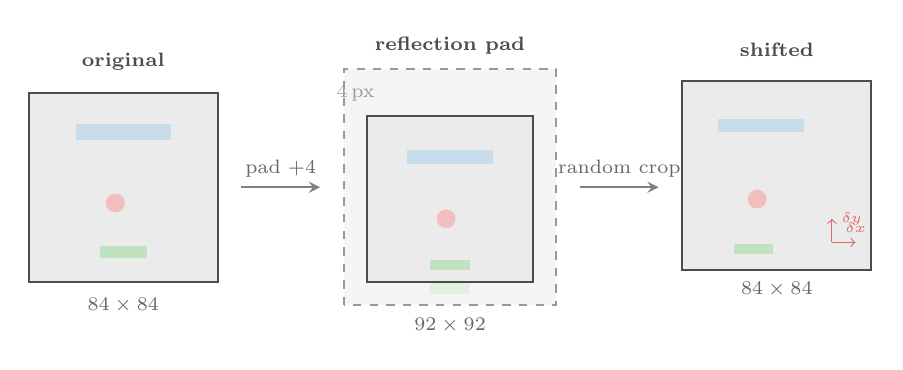
\begin{tikzpicture}[
    arr/.style={->, thick, >=stealth, black!50},
    lbl/.style={font=\scriptsize, text=black!60},
]

% === Panel 1: Original 84x84 ===
\draw[thick, black!70, fill=black!8]
    (0, 0) rectangle (2.4, 2.4);
% Content region schematic (simple game elements)
\fill[palA!25] (0.6, 1.8) rectangle (1.8, 2.0);  % top bar
\fill[palB!30] (1.1, 1.0) circle (0.12);          % ball
\fill[palC!30] (0.9, 0.3) rectangle (1.5, 0.45);  % paddle
\node[lbl] at (1.2, -0.3) {$84 \times 84$};
\node[font=\scriptsize\bfseries, text=black!70] at (1.2, 2.8)
    {original};

% Arrow 1
\draw[arr] (2.7, 1.2) -- node[above, lbl] {pad $+4$} (3.7, 1.2);

% === Panel 2: Padded 92x92 ===
% Padding region (lighter)
\draw[thick, black!40, fill=black!4, dashed]
    (4.0, -0.3) rectangle (6.7, 2.7);
% Original content region inside padding
\draw[thick, black!70, fill=black!8]
    (4.3, 0.0) rectangle (6.4, 2.1);
% Same game elements (shifted inward)
\fill[palA!25] (4.8, 1.5) rectangle (5.9, 1.67);
\fill[palB!30] (5.3, 0.8) circle (0.12);
\fill[palC!30] (5.1, 0.15) rectangle (5.6, 0.28);
% Reflection hint (mirrored paddle at bottom edge)
\fill[palC!15] (5.1, -0.15) rectangle (5.6, -0.02);
% Dimension labels
\node[lbl] at (5.35, -0.55) {$92 \times 92$};
% Padding annotation
\node[lbl, text=black!40] at (4.15, 2.4) {4\,px};
\node[font=\scriptsize\bfseries, text=black!70] at (5.35, 3.0)
    {reflection pad};

% Arrow 2
\draw[arr] (7.0, 1.2) -- node[above, lbl] {random crop} (8.0, 1.2);

% === Panel 3: Cropped 84x84 (shifted) ===
% Show a slightly offset crop
\draw[thick, black!70, fill=black!8]
    (8.3, 0.15) rectangle (10.7, 2.55);
% Same elements but shifted by ~2px equivalent
\fill[palA!25] (8.75, 1.9) rectangle (9.85, 2.07);
\fill[palB!30] (9.25, 1.05) circle (0.12);
\fill[palC!30] (8.95, 0.35) rectangle (9.45, 0.48);
\node[lbl] at (9.5, -0.1) {$84 \times 84$};
\node[font=\scriptsize\bfseries, text=black!70] at (9.5, 2.95)
    {shifted};

% Offset annotation (small arrows showing dx, dy)
\draw[->, thin, palB!70] (10.2, 0.5) -- (10.2, 0.8)
    node[right, font=\tiny, text=palB!70] {$\delta y$};
\draw[->, thin, palB!70] (10.2, 0.5) -- (10.5, 0.5)
    node[above, font=\tiny, text=palB!70] {$\delta x$};

\end{tikzpicture}
\caption{Random shift augmentation. The $84 \times 84$ frame is
  padded by 4 pixels on each side using reflection, then randomly
  cropped back to $84 \times 84$, producing a small spatial shift.}
\label{fig:random-shift}
\end{figure}
